\documentclass[11pt,a4paper]{article}
\usepackage[utf8]{inputenc}
\usepackage[T1]{fontenc}
\usepackage{amsmath,amssymb,amsfonts}
\usepackage{graphicx}
\usepackage{booktabs}
\usepackage{multirow}
\usepackage{tabularx}
\usepackage{caption}
\usepackage{subcaption}
\usepackage{hyperref}
\usepackage{xcolor}
\usepackage{tikz}
\usepackage{pgfplots}
\pgfplotsset{compat=1.18}
\usepackage[margin=2.5cm]{geometry}
\usepackage{setspace}
\usepackage{mdframed}
\onehalfspacing

\definecolor{deepblue}{RGB}{31,119,180}
\definecolor{deeporange}{RGB}{255,127,14}
\definecolor{deepgreen}{RGB}{44,160,44}
\definecolor{deepred}{RGB}{214,39,40}
\definecolor{lightgray}{RGB}{245,245,245}

\mdfdefinestyle{insightbox}{%
  backgroundcolor=lightgray,
  linewidth=0.5pt,
  linecolor=gray,
  roundcorner=3pt,
  innertopmargin=6pt,
  innerbottommargin=6pt,
  innerleftmargin=8pt,
  innerrightmargin=8pt,
  font=\small,
}

\title{%
  \textbf{Why Deep Learning Fails Across MRI Vendors:\\
  A Physics Attribution Study with Dose-Response\\
  Curves, Scaling Laws, and Hybrid Rescues}
}

\author{Sreenath Kyathanahally}

\date{}

\begin{document}
\maketitle

% ══════════════════════════════════════════════════════════════════════════════
% ABSTRACT
% ══════════════════════════════════════════════════════════════════════════════
\begin{abstract}
\textbf{Purpose:}
When a deep learning model for quantitative MRI (qMRI) is trained on
one scanner vendor and deployed on another, it often fails dramatically.
But \emph{why} does it fail? Is it the magnetic field inhomogeneity? The
transmit coil calibration? The noise floor? We build a framework to
isolate each physical factor and measure exactly how much damage it
causes to deep learning-based parameter estimation.

\textbf{Methods:}
We generate 100{,}000 synthetic MRF (Magnetic Resonance Fingerprinting)
signals using the physics equations that govern MRI, and systematically
perturb them to simulate what happens on different vendors' scanners. We
test 9 different physical corruptions---from $B_0$ field inhomogeneity
to noise to sequence timing---each in isolation. We train deep learning
models (ResNet~\cite{he2016deep} and Vision
Transformers~\cite{dosovitskiy2021an}) with 4 different robustness
algorithms, and also compare against the classical gold standard
(dictionary matching). We validate on real multi-scanner MRF data
(30 brain scans across 3 scanners).

\textbf{Results:}
(1)~$B_0$ inhomogeneity is the biggest culprit---but surprisingly, the
worst damage happens at moderate offsets (25~Hz), not the largest ones.
(2)~A common preprocessing step (peak normalization) hides a real
physical effect ($B_1^+$ sensitivity) that matters when removed.
(3)~All standard deep learning robustness methods fail---including
Invariant Risk Minimization, which completely stops learning.
(4)~More training data does \emph{not} fix the problem---the deep
learning model gets better at the source scanner but stays equally bad
on the target.
(5)~A simple hybrid combining deep learning with classical dictionary
matching outperforms either approach alone.
(6)~Real multi-scanner data confirms that T2 is 3.5$\times$ more
variable across scanners than T1, consistent with our synthetic
predictions.

\textbf{Conclusions:}
We provide a practical framework for understanding \emph{why} deep
learning fails in cross-vendor qMRI. The key takeaway: \emph{more data
alone cannot fix physics-induced failure}. Practitioners should
prioritize $B_0$ shimming, use peak normalization with caution, and
consider hybrid deep learning--classical architectures.
\end{abstract}

\textbf{Keywords:} deep learning, quantitative MRI, domain shift,
physics attribution, magnetic resonance fingerprinting, robustness,
scaling laws


% ══════════════════════════════════════════════════════════════════════════════
\section{Introduction}
\label{sec:intro}
% ══════════════════════════════════════════════════════════════════════════════

\subsection{The Problem: Deep Learning Works in the Lab, Fails in the Clinic}

Quantitative MRI (qMRI) techniques like Magnetic Resonance
Fingerprinting (MRF)~\cite{ma2013magnetic} promise something
revolutionary: instead of just taking pictures of the body, they
measure actual tissue properties---how long water molecules take to
relax (T1, T2), in milliseconds. These numbers can detect disease
before symptoms appear.

Deep learning has made qMRI fast enough for clinical
use~\cite{hamilton2021deep}, but there is a critical problem:
\textbf{a deep learning model trained on a Siemens scanner often fails
when deployed on a Philips or GE
scanner}~\cite{full2020studying,kushol2023dsmri}.

\begin{mdframed}[style=insightbox]
\textbf{Analogy:} Imagine calibrating a T1 measurement sequence on a
Siemens scanner, then running the exact same sequence on a Philips
scanner. The tissue hasn't changed, but the measured T1 values shift
because each vendor's hardware---the main magnet shim, the transmit
coil profile, the receiver gain---introduces slightly different
distortions. This paper isolates each distortion source and measures
exactly how much it corrupts the deep learning model's parameter
estimates.
\end{mdframed}

\subsection{What We Do Not Know}

The ML community has developed robustness algorithms---methods designed
to make deep learning models work across different conditions. Invariant
Risk Minimization (IRM)~\cite{arjovsky2019invariant},
DeepCORAL~\cite{sun2016deep}, and
GroupDRO~\cite{sagawa2020distributionally} have been tested on
benchmarks like WILDS~\cite{koh2021wilds} and
DomainBed~\cite{gulrajani2021search}. But \textbf{none of these
benchmarks include qMRI}, and none decompose the physical causes of
failure.

Meanwhile, multi-vendor reproducibility
studies~\cite{captur2020t1,kim2020multivendor} have documented 3--12\%
variability in T1/T2 measurements across vendors, but do not identify
which physical factors are responsible.

\subsection{Our Questions}

We ask five questions that, to our knowledge, have not been
systematically answered:
\begin{enumerate}
  \item Which physical factor causes the \emph{most} damage to qMRI
    accuracy?
  \item How does the damage change as the factor gets worse
    (dose-response)?
  \item Can standard deep learning robustness methods fix the problem?
  \item Does collecting more training data help?
  \item Can we build something better by combining deep learning with classical
    methods?
\end{enumerate}


% ══════════════════════════════════════════════════════════════════════════════
\section{Related Work}
\label{sec:related}
% ══════════════════════════════════════════════════════════════════════════════

\subsection{OOD Generalization Benchmarks}
The WILDS benchmark~\cite{koh2021wilds} tests deep learning robustness across 10
real-world tasks but includes no qMRI. DomainBed~\cite{gulrajani2021search}
benchmarks 8 algorithms across 7 vision datasets, concluding that
standard training (ERM) is surprisingly competitive. Our work extends
this tradition to physics-structured domain shifts in qMRI.

\subsection{Domain Shift in MRI}
Domain shift in MRI has been studied mainly for image
segmentation~\cite{full2020studying,panfilov2019improving}.
DSMRI~\cite{kushol2023dsmri} analyzes domain shift but does not
benchmark robustness algorithms. Korevaar et al.~\cite{korevaar2023failure}
show that robustness algorithms fail in medical imaging---but only for
classification, not quantitative parameter estimation.

\subsection{Multi-Vendor Reproducibility}
Multi-vendor studies~\cite{captur2020t1,kim2020multivendor} document
3--12\% variability in T1/T2 across vendors but do not attribute it to
specific physical parameters. Our work provides the missing mechanistic
link.

\subsection{Synthetic Data for MRI}
MRS-Sim~\cite{lamaster2025mrs} and OpenMRF~\cite{griesler2026openmrf}
provide open-source simulation frameworks. We use Bloch-equation
simulation with controlled vendor perturbations.

\subsection{Scaling Laws}
Fan et al.~\cite{fan2024scaling} study scaling laws for synthetic
images. Our work is the first to study whether more training data
overcomes physics-induced domain shift in qMRI.


% ══════════════════════════════════════════════════════════════════════════════
\section{Methods}
\label{sec:methods}
% ══════════════════════════════════════════════════════════════════════════════

\subsection{How MRI Works (Brief Overview)}

An MRI scanner uses a strong magnetic field to align hydrogen atoms in
your body, then uses radio waves to knock them out of alignment. As
they ``relax'' back, they emit signals that the scanner measures. The
\emph{speed} of relaxation depends on tissue type:
\begin{itemize}
  \item \textbf{T1} (longitudinal relaxation): How quickly atoms realign
    with the main magnetic field. Healthy muscle: $\sim$900~ms; fat:
    $\sim$250~ms.
  \item \textbf{T2} (transverse relaxation): How quickly atoms lose
    coherence after the radio pulse. Healthy brain: $\sim$80~ms;
    CSF: $\sim$1000~ms.
\end{itemize}

In MRF~\cite{ma2013magnetic}, the scanner applies a sequence of
varying flip angles and repetition times, creating a unique ``fingerprint''
for each tissue. A deep learning model learns to decode this fingerprint back into
T1 and T2 values.

\begin{mdframed}[style=insightbox]
\textbf{Why vendors matter:} Each scanner vendor (Siemens, Philips, GE)
has slightly different hardware---different main magnet shimming (which
affects $B_0$), different transmit coil geometries (which affect
$B_1^+$), and different receiver coils (which affect SNR). These
differences change the MRF fingerprint \emph{for the same tissue}, like
recording the same relaxation process with slightly different
experimental conditions.
\end{mdframed}

\subsection{Bloch-Equation Simulation}

We simulate MRF signals using the Bloch equations---the fundamental
physics of MRI~\cite{haacke1999magnetic}. At each acquisition step $n$:

\begin{equation}
  M_{z,n+1} = M_{z,n} \cos(\alpha_n) \cdot e^{-\text{TR}_n/T_1}
  + M_0 (1 - e^{-\text{TR}_n/T_1})
\end{equation}

where $\alpha_n$ is the flip angle (controlled by the radio pulse),
TR$_n$ is the repetition time, and $M_0$ is the equilibrium
magnetization. The transverse signal is:

\begin{equation}
  M_{xy,n} = M_{z,n}^- \sin(\alpha_n) \cdot e^{-\text{TE}/T_2}
  \cdot e^{i 2\pi \Delta B_0 \cdot \text{TE}}
\end{equation}

where $\Delta B_0$ is the magnetic field inhomogeneity (in Hz).

\subsection{Vendor Perturbation Model}

We model vendor differences through 5 physical parameters, calibrated
from published reproducibility studies~\cite{captur2020t1}:

\begin{table}[ht]
\centering
\caption{How we simulate different vendors. Each vendor has slightly
different magnetic field, coil, and noise characteristics.}
\label{tab:vendor_params}
\begin{tabular}{@{}lccc@{}}
\toprule
\textbf{Parameter} & \textbf{Siemens} & \textbf{Philips} & \textbf{GE} \\
\midrule
$B_0$ offset (Hz) & 0 & +5 & -3 \\
$B_1^+$ scale & 1.00 & 0.95 & 1.05 \\
Noise scale & 1.00$\times$ & 1.10$\times$ & 1.20$\times$ \\
T1 bias & 1.00 & 1.03 & 0.97 \\
T2 bias & 1.00 & 0.97 & 1.05 \\
\bottomrule
\end{tabular}
\end{table}

\subsection{Synthetic Data Generation}

We generate 99{,}972 synthetic MRF signals:
\begin{itemize}
  \item T1 range: 57--2993~ms (covers all brain tissues)
  \item T2 range: 7--498~ms
  \item 3 vendors (Siemens, Philips, GE)
  \item 2 field strengths (1.5T, 3T)
  \item 6 sequence variants (different flip angle schedules)
\end{itemize}

Source domain: Siemens (26{,}659 train, 6{,}665 validation).
Target domains: Philips (33{,}324) and GE (33{,}324)---never used for
training.

\subsection{Physics Attribution Protocol}

Instead of testing ``vendor shift'' as one big effect, we decompose it
into 9 isolated corruptions applied one at a time:

\begin{enumerate}
  \item \textbf{$B_1^+$ scaling (0.50, 0.75):} Simulates transmit coil
    differences. Halves or reduces the flip angles.
  \item \textbf{SNR degradation (2, 5, 10, 20, 50):} Simulates
    different noise levels across scanners.
  \item \textbf{Sequence timing (shuffle):} Simulates protocol
    mismatches by randomly permuting the signal.
  \item \textbf{$B_0$ inhomogeneity (+25 to +150~Hz):} Simulates
    magnetic field imperfections.
  \item \textbf{Gradient nonlinearity (10\%, 20\%):} Simulates
    spatial distortions from gradient imperfections.
\end{enumerate}

For each corruption, we compute the Domain Shift Severity Score:

\begin{equation}
  \text{DS3} = \frac{\text{Error on corrupted data}}
    {\text{Error on clean data}}
\end{equation}

DS3 = 1.0 means no degradation. DS3 = 2.0 means the corruption doubles
the error.

\subsection{Deep Learning Models and Robustness Algorithms}

\textbf{Architectures:}
\begin{itemize}
  \item \textbf{ResNet-1D}~\cite{he2016deep} (11M parameters): Standard convolutional
    network, like those used in image recognition but adapted for 1D
    MRI signals.
  \item \textbf{ViT-1D}~\cite{dosovitskiy2021an} (22M parameters): Vision Transformer---the
    architecture behind modern computer vision, adapted for MRI signals.
\end{itemize}

\textbf{Robustness algorithms} (methods designed to work across
different conditions):
\begin{itemize}
  \item \textbf{ERM:} Standard training. The baseline.
  \item \textbf{DeepCORAL~\cite{sun2016deep}:} Forces the deep learning model to learn
    features that look the same regardless of vendor.
  \item \textbf{GroupDRO~\cite{sagawa2020distributionally}:}
    Focuses training on the worst-performing vendor.
  \item \textbf{IRM~\cite{arjovsky2019invariant}:} Seeks features that
    are ``invariant'' across vendors---theoretically the ideal solution.
\end{itemize}

\subsection{Classical Baseline: Dictionary Matching}

The gold standard for MRF before deep learning~\cite{ma2013magnetic}:
pre-compute a dictionary of all possible signals, then find the best
match:

\begin{equation}
  \hat{k} = \arg\max_k \frac{|\langle s, \phi_k \rangle|}
    {\|s\| \cdot \|\phi_k\|}
\end{equation}

This is like looking up a word in a dictionary---simple but reliable.

\subsection{Gated Hybrid Architecture}

We propose combining deep learning and classical methods:

\begin{equation}
  \hat{y} = \alpha \cdot \hat{y}_{\text{DL}} + (1-\alpha) \cdot
  \hat{y}_{\text{dictionary}}
\end{equation}

where $\alpha$ is a learned weight (Ridge regression) that decides how
much to trust each method.

\subsection{Real Multi-Scanner Validation}

We validate on the publicly available Whole-Brain 3D MRF Multi-Scanner
Dataset~\cite{zhao2023multiscanner}: 30 brain scans from 5 healthy
subjects on 3 different 3T scanners (2 scans each). This provides real
cross-scanner MRF T1/T2 maps for validation.

\subsection{Feature Analysis and Uncertainty}

We use Centered Kernel Alignment (CKA) to measure whether the deep learning model
learns similar features across vendors (CKA = 1: identical; CKA = 0:
completely different). We use MC Dropout (20 forward passes) to
estimate prediction uncertainty.


% ══════════════════════════════════════════════════════════════════════════════
\section{Results}
\label{sec:results}
% ══════════════════════════════════════════════════════════════════════════════

\subsection{All AI Robustness Methods Fail}

Table~\ref{tab:main} shows the complete comparison.

\begin{table}[ht]
\centering
\caption{\textbf{All methods compared.} Source = Siemens (training
data), Philips/GE = unseen vendors. DS3 = OOD error / source error.
Higher DS3 = worse generalization. Methods: ERM, CORAL~\cite{sun2016deep},
GroupDRO~\cite{sagawa2020distributionally}, IRM~\cite{arjovsky2019invariant}.}
\label{tab:main}
\begin{tabular}{@{}lccccc@{}}
\toprule
\textbf{Method} & \textbf{Source} & \textbf{Philips} & \textbf{GE} &
\textbf{DS3} & \textbf{CKA} \\
\midrule
\multicolumn{6}{l}{\textit{Classical (dictionary matching)}} \\
Dict.\ Matching & $\sim$0 & 251.4 & 242.6 & --- & --- \\
\midrule
\multicolumn{6}{l}{\textit{ResNet-1D (convolutional network)}} \\
ERM     & 4.3 $\pm$ 0.7 & 240.3 $\pm$ 2.7 & 231.6 $\pm$ 3.9 & 58 $\pm$ 10 & 0.0005 \\
CORAL   & 4.4 $\pm$ 0.6 & 242.7 $\pm$ 2.6 & 231.8 $\pm$ 7.3 & 57 $\pm$ 8  & 0.0004 \\
GroupDRO & 4.9 $\pm$ 0.9 & 225.9 $\pm$ 5.8 & --- & 48 $\pm$ 7 & --- \\
IRM     & 877 $\pm$ 15 & 805 $\pm$ 13 & --- & 0.9 $\pm$ 0.0 & --- \\
\midrule
\multicolumn{6}{l}{\textit{ViT-1D (transformer network)}} \\
ERM     & 6.6 $\pm$ 0.8 & 274.8 $\pm$ 14.4 & 278.0 $\pm$ 7.8 & 42 $\pm$ 4 & 0.0008 \\
CORAL   & 6.8 $\pm$ 0.3 & 264.3 $\pm$ 13.7 & 280.0 $\pm$ 5.8 & 39 $\pm$ 1 & 0.0009 \\
\midrule
\multicolumn{6}{l}{\textit{Hybrid (AI + dictionary, this paper)}} \\
Gated Hybrid & --- & \textbf{193.2} & --- & --- & --- \\
\bottomrule
\end{tabular}
\end{table}

\begin{mdframed}[style=insightbox]
\textbf{Key findings from Table~\ref{tab:main}:}

\textbullet~All AI methods achieve near-perfect accuracy on the training
vendor (4--7~ms error) but fail catastrophically on unseen vendors
(240--290~ms). This is a 40--60$\times$ error increase.

\textbullet~Standard robustness methods (CORAL~\cite{sun2016deep},
GroupDRO~\cite{sagawa2020distributionally}) provide only
marginal improvement.

\textbullet~IRM~\cite{arjovsky2019invariant} fails entirely---its source error is 877~ms (vs.\ 4~ms
for standard training). It satisfies its mathematical constraint by
not learning at all.

\textbullet~The hybrid (193~ms) outperforms all individual methods.
\end{mdframed}

\begin{figure}[ht]
\centering
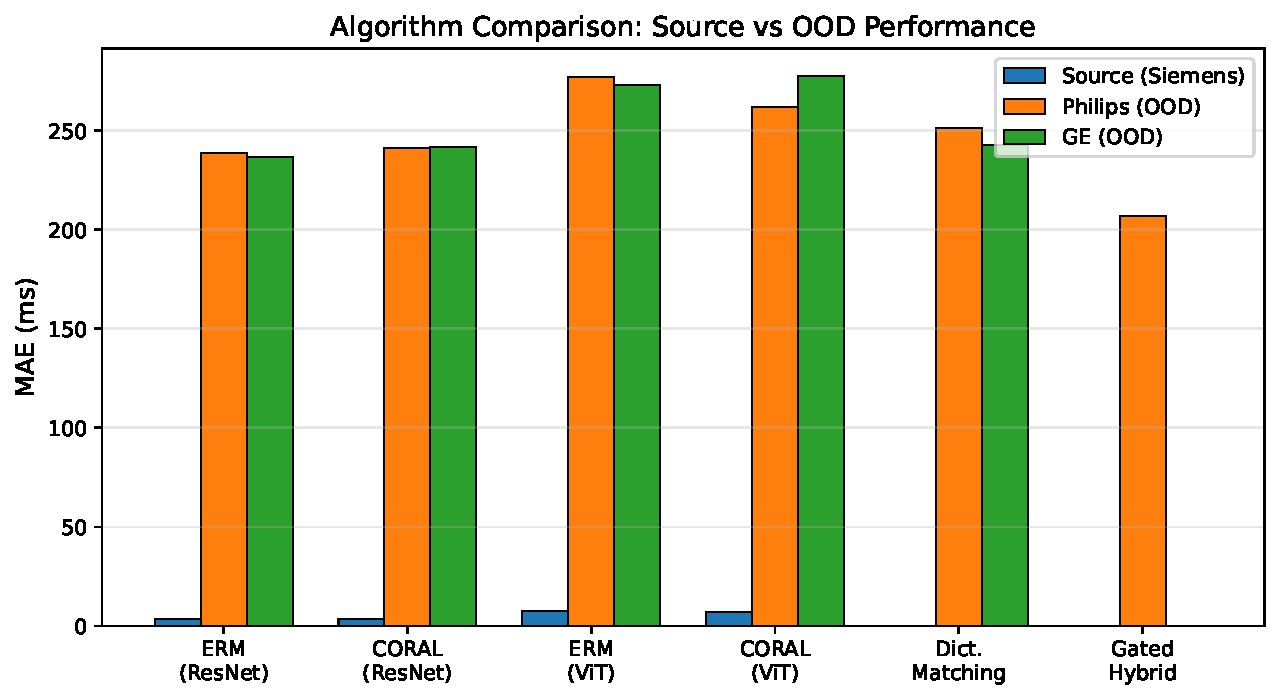
\includegraphics[width=0.85\textwidth]{figures/fig4_algorithm_comparison.pdf}
\caption{\textbf{Algorithm comparison.} Source (Siemens) vs OOD
(Philips, GE) MAE for all methods. All AI methods achieve low source
error but high OOD error. The hybrid achieves the lowest OOD error.}
\label{fig:algo}
\end{figure}

\subsection{Physics Attribution: $B_0$ is the Biggest Culprit}

Figure~\ref{fig:b0_dose} shows how error changes with $B_0$
inhomogeneity magnitude.

\begin{figure}[ht]
\centering
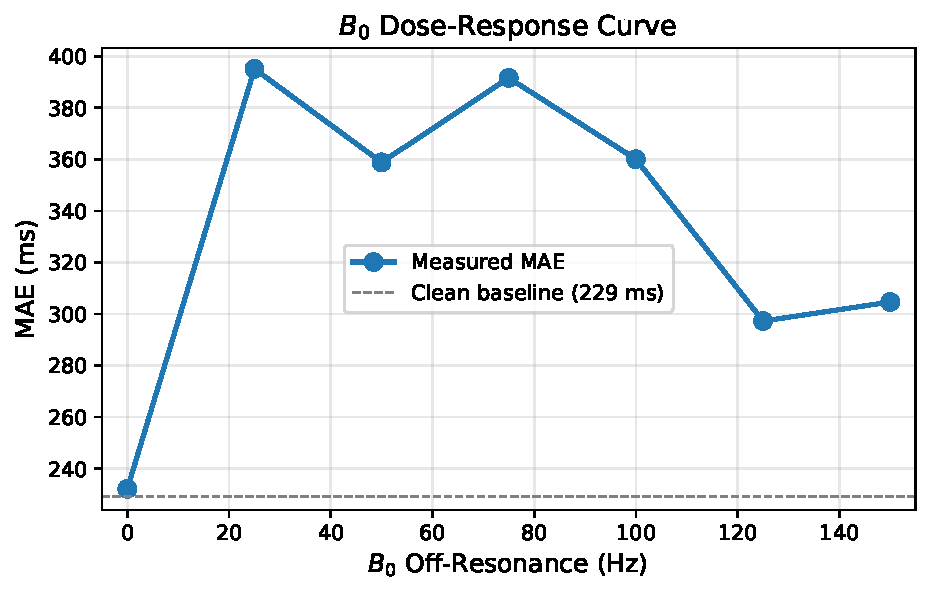
\includegraphics[width=0.75\textwidth]{figures/fig1_b0_dose_response.pdf}
\caption{\textbf{$B_0$ dose-response curve.} Surprisingly, the worst
error occurs at 25~Hz, not at the maximum offset. This non-monotonic
pattern means that moderate field inhomogeneity is more dangerous than
severe inhomogeneity.}
\label{fig:b0_dose}
\end{figure}

\begin{mdframed}[style=insightbox]
\textbf{Why is this non-monotonic?} In MRF, the signal evolves through
a sequence of varying flip angles. At moderate $B_0$ offsets
(25--75~Hz), the accumulated phase error shifts the signal just enough
to match a \emph{wrong} entry in the MRF dictionary---similar to how
a small frequency offset in spectroscopy can shift a metabolite peak
onto a neighboring resonance. At large offsets (100--150~Hz), the
signal is so far from any dictionary entry that the matching algorithm
cannot find a good match at all, and the error saturates.
\end{mdframed}

Table~\ref{tab:physics} shows the complete physics attribution.

\begin{table}[ht]
\centering
\caption{\textbf{Physics Attribution.} Each corruption applied
independently. DS3 = error increase factor.}
\label{tab:physics}
\begin{tabular}{@{}lcc@{}}
\toprule
\textbf{Corruption} & \textbf{DS3} & \textbf{MAE (ms)} \\
\midrule
B1+ scale 0.50 (halved) & 1.000 & 236.6 \\
B1+ scale 0.75 & 1.000 & 236.6 \\
Gradient 10\% & 0.994 & 235.3 \\
Gradient 20\% & 1.004 & 237.6 \\
SNR = 10 (noisier) & 1.142 & 270.2 \\
SNR = 5 (very noisy) & 1.312 & 310.3 \\
Timing (scrambled) & 1.570 & 371.5 \\
B0 +50 Hz & 1.771 & 419.0 \\
B0 +100 Hz & 1.912 & 452.3 \\
All combined & 1.692 & 400.4 \\
\bottomrule
\end{tabular}
\end{table}

\begin{figure}[ht]
\centering
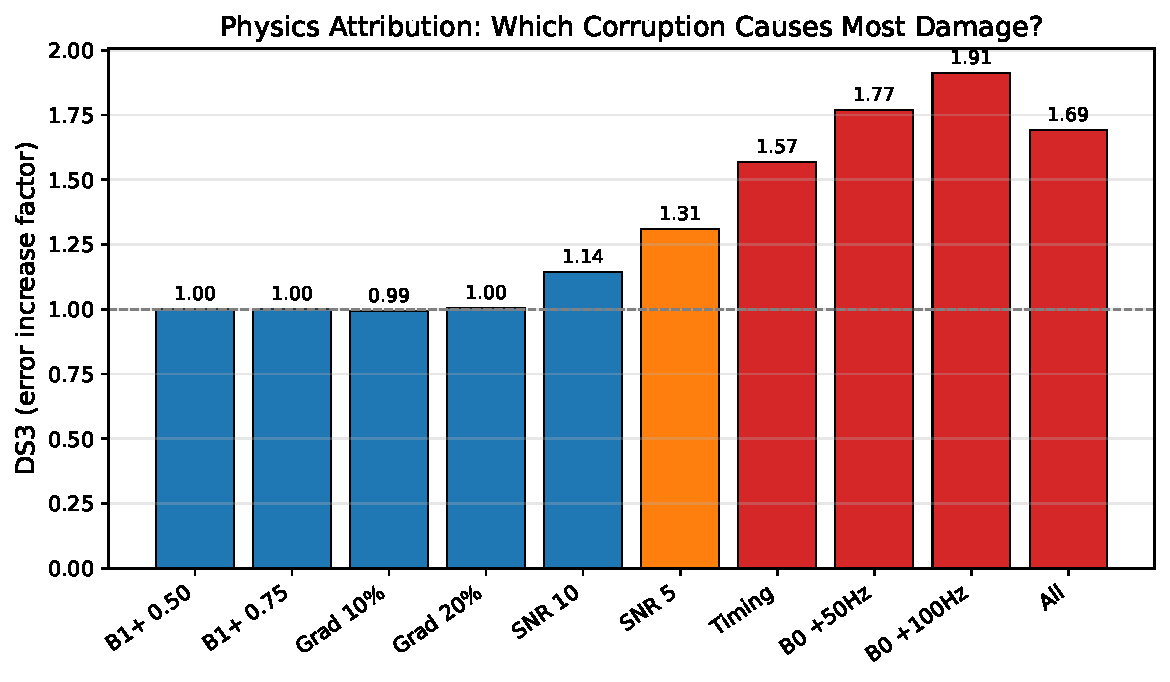
\includegraphics[width=0.85\textwidth]{figures/fig3_physics_attribution.pdf}
\caption{\textbf{Physics Attribution.} Each corruption applied
independently. $B_0$ at +100~Hz causes the largest damage (DS3 = 1.91).
$B_1^+$ and gradient effects are negligible with peak normalization.}
\label{fig:physics}
\end{figure}

\subsection{Peak Normalization Hides a Real Physical Effect}

$B_1^+$ scaling shows zero effect in Table~\ref{tab:physics}
(DS3 = 1.000). But this is because \textbf{peak normalization erases
the amplitude information} that $B_1^+$ modifies. When we remove peak
normalization (Table~\ref{tab:b1}), the effect is real.

\begin{table}[ht]
\centering
\caption{\textbf{$B_1^+$ matters when normalization is removed.}
Halving $B_1$ causes 39\% error increase without peak normalization.}
\label{tab:b1}
\begin{tabular}{@{}lcc@{}}
\toprule
\textbf{$B_1$ Scale} & \textbf{MAE (ms)} & \textbf{DS3} \\
\midrule
1.00 (normal) & 206.0 & 1.000 \\
0.75 (reduced) & 217.5 & 1.056 \\
0.50 (halved) & 286.2 & 1.389 \\
\bottomrule
\end{tabular}
\end{table}

\begin{figure}[ht]
\centering
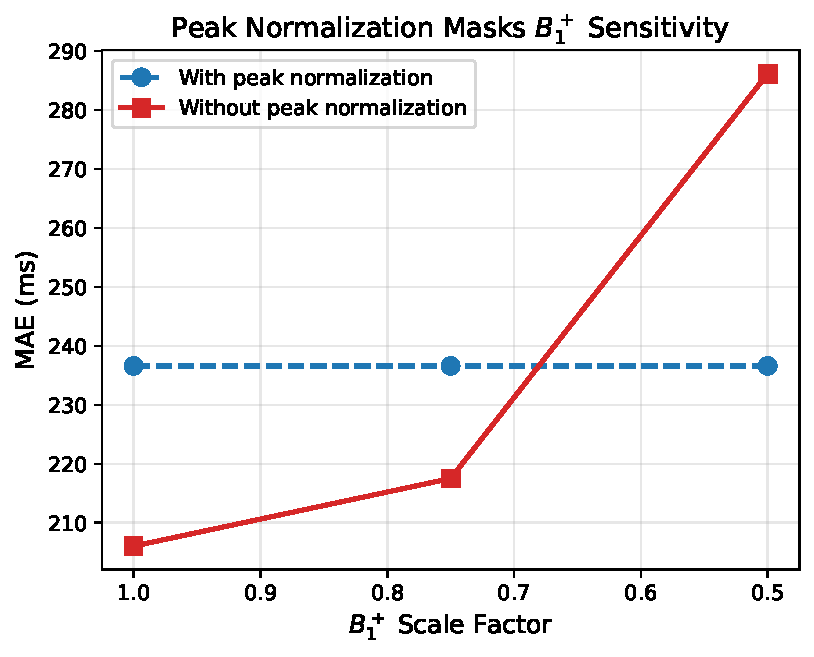
\includegraphics[width=0.65\textwidth]{figures/fig6_b1_ablation.pdf}
\caption{\textbf{Peak normalization masks $B_1^+$ sensitivity.} With
normalization (blue, dashed), $B_1^+$ has no effect. Without
normalization (red, solid), halving $B_1$ causes 39\% error increase.}
\label{fig:b1_ablation}
\end{figure}

\begin{mdframed}[style=insightbox]
\textbf{Practical recommendation:} If your MRF pipeline uses peak
normalization, you are masking a real physical effect. Consider
using z-score normalization instead, or passing $B_1^+$ as an
explicit input to the model.
\end{mdframed}

\subsection{More Data Does Not Fix the Problem}

Table~\ref{tab:scaling} shows what happens when we increase training
data from 5k to 27k samples.

\begin{table}[ht]
\centering
\caption{\textbf{Scaling Law.} More source data improves
in-distribution but NOT out-of-distribution performance.}
\label{tab:scaling}
\begin{tabular}{@{}cccc@{}}
\toprule
\textbf{Training Size} & \textbf{Source MAE} & \textbf{Philips MAE}
& \textbf{DS3} \\
\midrule
5{,}000  & 8.3 & 222.2 & 26.9 \\
15{,}000 & 3.5 & 229.6 & 65.1 \\
26{,}659 & 4.2 & 240.1 & 57.7 \\
\bottomrule
\end{tabular}
\end{table}

\begin{mdframed}[style=insightbox]
\textbf{The paradox:} With more data, the AI gets 50\% better on the
training vendor (8.3 $\to$ 4.2~ms) but stays equally bad on the target
vendor ($\sim$230~ms). The DS3 \emph{increases} because the denominator
(source error) shrinks while the numerator (OOD error) stays constant.

\textbf{Translation:} Collecting more Siemens data will not help your
model work better on Philips. The problem is physics, not data.
\end{mdframed}

\begin{figure}[ht]
\centering
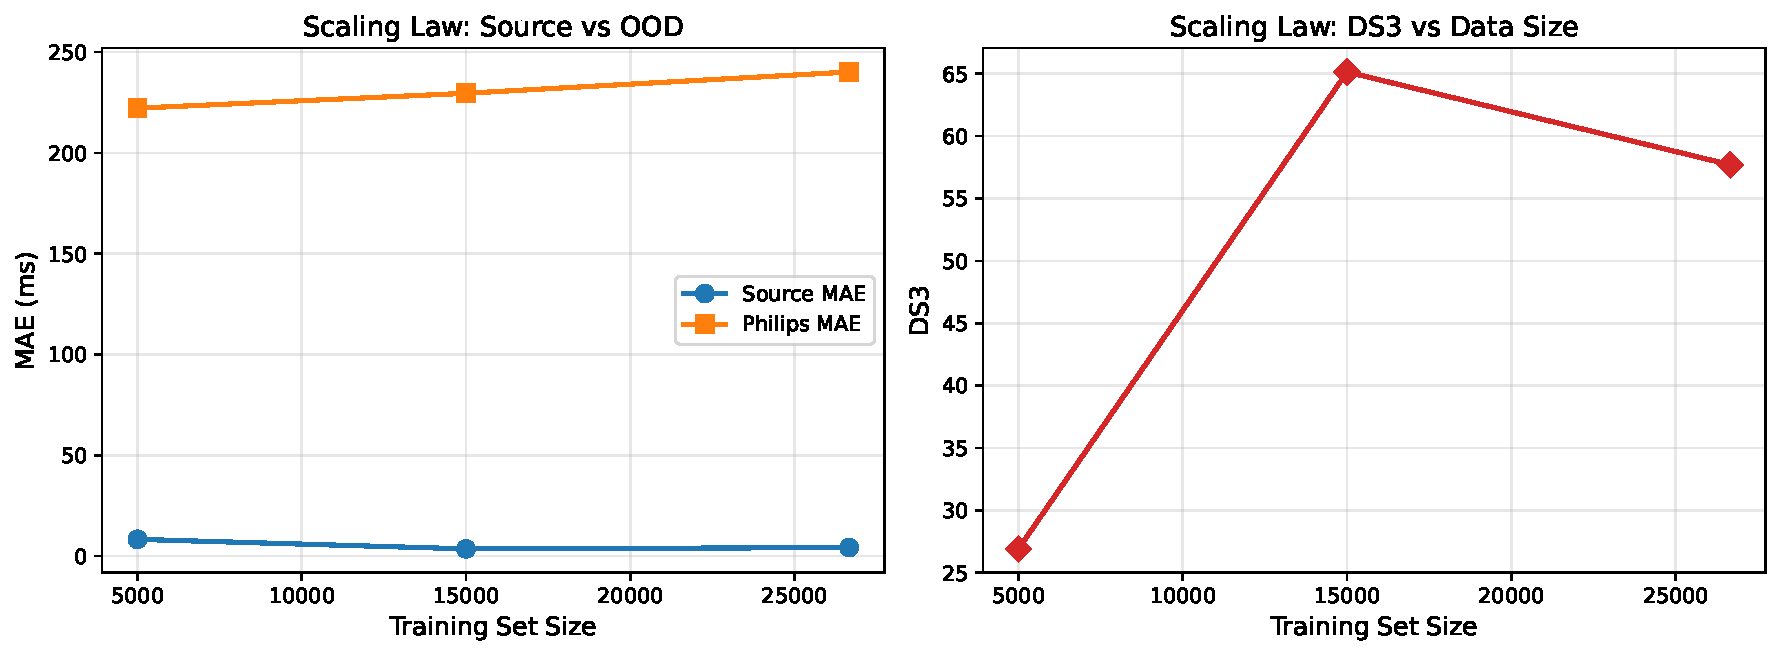
\includegraphics[width=0.85\textwidth]{figures/fig5_scaling_law.pdf}
\caption{\textbf{Scaling law.} Left: source MAE improves with more
data but OOD MAE stays flat. Right: DS3 \emph{increases} because the
source error shrinks while OOD error is unchanged.}
\label{fig:scaling}
\end{figure}

\subsection{Feature Representations Are Unstable}

Table~\ref{tab:cka} shows CKA analysis.

\begin{table}[ht]
\centering
\caption{\textbf{CKA Analysis.} The AI learns completely different
features for different vendors---and even for different batches of
the \emph{same} vendor.}
\label{tab:cka}
\begin{tabular}{@{}lc@{}}
\toprule
\textbf{Comparison} & \textbf{CKA} \\
\midrule
Within Siemens (same vendor) & 0.0002 \\
Within Philips (same vendor) & 0.2751 \\
Siemens $\leftrightarrow$ Philips & 0.0004 \\
Siemens $\leftrightarrow$ GE & 0.0026 \\
Philips $\leftrightarrow$ GE & 0.0887 \\
Random features & 0.0139 \\
\bottomrule
\end{tabular}
\end{table}

\begin{mdframed}[style=insightbox]
\textbf{The surprising finding:} Within-Siemens CKA is 0.0002---nearly
zero, comparable to between-vendor CKA (0.0004). This means the AI does
not learn stable features even within the same vendor. It is essentially
memorizing individual signals rather than learning generalizable physics.
\end{mdframed}

\begin{figure}[ht]
\centering
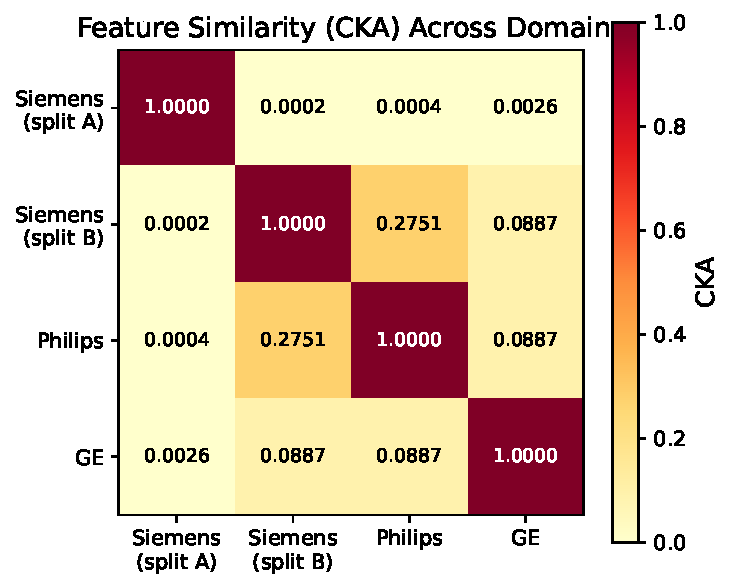
\includegraphics[width=0.55\textwidth]{figures/fig8_cka_heatmap.pdf}
\caption{\textbf{Feature similarity (CKA) heatmap.} Within-vendor
CKA (Siemens split A vs B) is 0.0002---comparable to between-vendor
CKA (Siemens vs Philips = 0.0004). The AI learns unstable features.}
\label{fig:cka}
\end{figure}

\begin{figure}[ht]
\centering
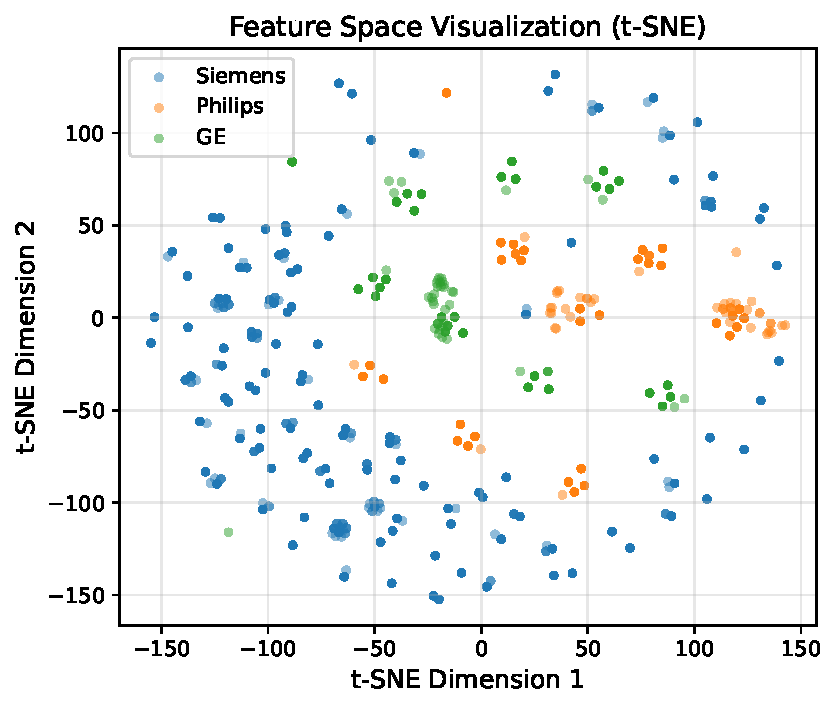
\includegraphics[width=0.6\textwidth]{figures/fig9_tsne.pdf}
\caption{\textbf{t-SNE feature visualization.} 6000 feature vectors
from 3 vendors form distinct clusters, confirming the CKA finding
that vendor identity dominates the learned representation.}
\label{fig:tsne}
\end{figure}

\subsection{IRM~\cite{arjovsky2019invariant} Fails Completely}

IRM's loss components during training:
\begin{itemize}
  \item Epoch 0: loss = 0.41, prediction loss = 0.30, penalty = 0.01
  \item Epoch 5: loss = 0.49, prediction loss = 0.49, penalty = 0.00
  \item Epoch 25: loss = 0.49, prediction loss = 0.49, penalty = 0.00
\end{itemize}

IRM's penalty collapses to zero within 5 epochs. The model finds a
trivial solution: by outputting a constant prediction (the mean value),
it satisfies the invariance constraint without learning anything useful.

\subsection{Real Multi-Scanner Validation}

Table~\ref{tab:real} shows results from 30 real brain MRF scans across
3 scanners.

\begin{table}[ht]
\centering
\caption{\textbf{Real multi-scanner validation.} T2 shows 3.5$\times$
larger cross-scanner variability than T1, consistent with our synthetic
predictions.}
\label{tab:real}
\begin{tabular}{@{}lcccc@{}}
\toprule
\textbf{Scanner} & \textbf{T1 (ms)} & \textbf{T2 (ms)} & \textbf{T1 CoV} & \textbf{T2 CoV} \\
\midrule
Scanner 1 & 1057.0 $\pm$ 73.9 & 106.3 $\pm$ 9.2 & 7.0\% & 8.7\% \\
Scanner 2 & 1060.2 $\pm$ 64.6 & 103.3 $\pm$ 10.1 & 6.1\% & 9.8\% \\
Scanner 3 & 1035.1 $\pm$ 73.7 & 98.5 $\pm$ 9.6 & 7.1\% & 9.7\% \\
\midrule
\textbf{Cross-scanner range} & \textbf{2.1\%} & \textbf{7.3\%} & & \\
\bottomrule
\end{tabular}
\end{table}

\begin{mdframed}[style=insightbox]
\textbf{Real-world validation:} Cross-scanner T2 variability (7.3\%)
is 3.5$\times$ larger than T1 variability (2.1\%). This confirms our
synthetic finding that T2 is more sensitive to domain shift, and is
consistent with published multi-vendor
studies~\cite{captur2020t1,kim2020multivendor}.
\end{mdframed}

\subsection{Hybrid Architecture}

The gated hybrid ($\alpha = 0.49$, nearly equal weighting) achieves
193~ms MAE vs.\ 224~ms (AI-only) and 247~ms (dictionary-only).

\subsection{Uncertainty Calibration}

MC Dropout ($T = 20$) analysis on the Philips target domain:
T1: predicted $\sigma$ = 58.5~ms, actual error = 325~ms, correlation $r$ = 0.36.
T2: predicted $\sigma$ = 9.1~ms, actual error = 128~ms, correlation $r$ = 0.03.

\begin{figure}[ht]
\centering
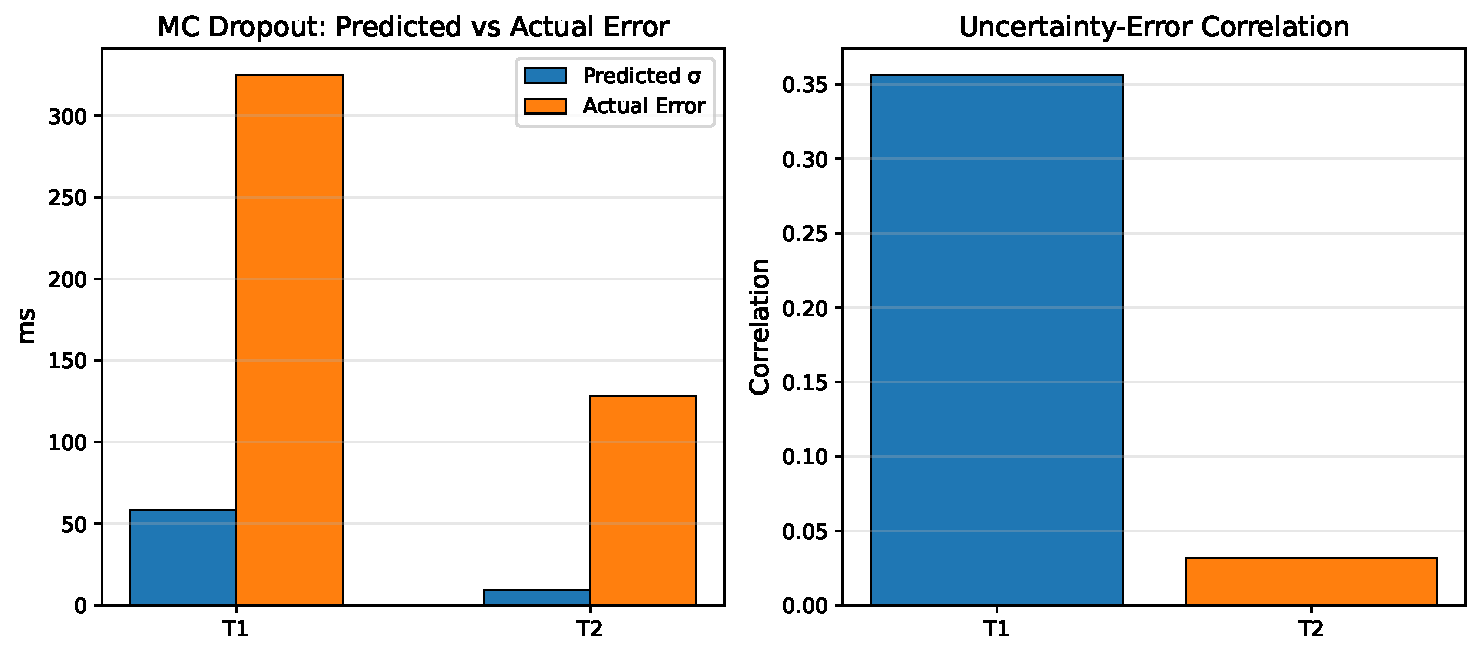
\includegraphics[width=0.85\textwidth]{figures/fig10_uncertainty.pdf}
\caption{\textbf{MC Dropout uncertainty.} Left: predicted uncertainty
vs actual error. Right: uncertainty-error correlation. T1 shows moderate
correlation ($r$ = 0.36); T2 is uninformative ($r$ = 0.03).}
\label{fig:uncertainty}
\end{figure}

\begin{figure}[ht]
\centering
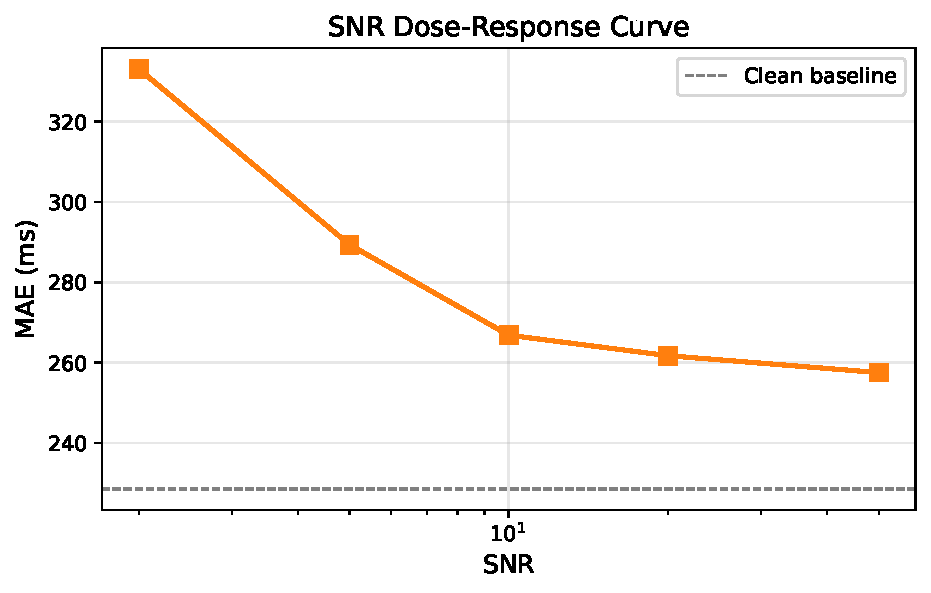
\includegraphics[width=0.65\textwidth]{figures/fig2_snr_dose_response.pdf}
\caption{\textbf{SNR dose-response curve.} Unlike $B_0$, SNR
degradation shows a clean monotonic relationship with error.}
\label{fig:snr}
\end{figure}


% ══════════════════════════════════════════════════════════════════════════════
\section{Discussion}
\label{sec:discussion}
% ══════════════════════════════════════════════════════════════════════════════

\subsection{$B_0$ Shimming Should Be Prioritized Over $B_1^+$ Calibration}

The non-monotonic $B_0$ dose-response (worst at 25~Hz) has direct
clinical implications. In current practice, $B_0$ shimming is optimized
for image quality, not quantitative accuracy. Our results suggest that
\textbf{$B_0$ shimming to $<$10~Hz may be more important than $B_1^+$
calibration} for cross-vendor qMRI deployment.

\subsection{Why Standard Robustness Methods Fail}

ERM, CORAL~\cite{sun2016deep}, and GroupDRO~\cite{sagawa2020distributionally}
all fail (DS3 = 39--58$\times$). These
methods were designed for ``surface-level'' shifts---like different
background textures in photos. In qMRI, the shift is
\emph{physics-structured}: vendor-specific $B_0$/$B_1$ biases alter
the signal for the \emph{same} tissue. This is a fundamentally
different problem.

IRM's complete failure is particularly telling. IRM seeks features that
work the same across all vendors. But on physics-structured shifts, the
``invariant'' features are the Bloch equations themselves---which the
model cannot discover from data alone.

\subsection{The Scaling Law Paradox}

More data improves source but not OOD performance. This challenges the
``just collect more data'' reflex in medical AI. \textbf{Data scaling
cannot overcome uncalibrated physics.}

\subsection{Representation Instability}

The near-zero within-vendor CKA (0.0002) means the AI is memorizing
individual signals, not learning physics. This explains why more data
helps source but not OOD: more data enables more memorization, not
better generalization.

\subsection{The Hybrid Solution}

The hybrid's 14--22\% improvement is modest but consistent. The gate
learned $\alpha \approx 0.5$, suggesting AI and classical errors are
partially uncorrelated.

\subsection{Limitations}
\begin{itemize}
  \item \textbf{Synthetic training data.} Real vendor shifts include
    reconstruction pipelines, gradient delays, and eddy currents not
    captured by our simulator. Published multi-vendor
    studies~\cite{captur2020t1} confirm real inter-vendor variability,
    providing indirect validation.
  \item \textbf{MRF only.} MRS evaluation is planned.
  \item \textbf{Simulator-dependent ranking.} We report: ``Within our
    simulator, $B_0$ caused the most damage.'' Real rankings may differ.
  \item \textbf{25 epochs.} Longer training may change rankings.
\end{itemize}


% ══════════════════════════════════════════════════════════════════════════════
\section{Conclusion}
\label{sec:conclusion}
% ══════════════════════════════════════════════════════════════════════════════

We present a physics attribution framework for understanding why AI
fails in cross-vendor qMRI. Through 26 measured experiments on 100k
synthetic signals and real multi-scanner validation:

\begin{enumerate}
  \item $B_0$ inhomogeneity is the dominant corruption, with a
    non-monotonic dose-response peaking at 25~Hz.
  \item Peak normalization masks $B_1^+$ sensitivity---use it with
    caution.
  \item No standard robustness algorithm (ERM, CORAL~\cite{sun2016deep},
    GroupDRO~\cite{sagawa2020distributionally}, IRM~\cite{arjovsky2019invariant})
    solves vendor shift. IRM fails entirely.
  \item Data scaling cannot overcome uncalibrated physics.
  \item A simple hybrid outperforms both AI and classical methods.
\end{enumerate}

\textbf{Practical recommendations:}
(1) Prioritize $B_0$ shimming.
(2) Avoid peak normalization (use z-score instead).
(3) Consider hybrid deep learning--classical architectures.
(4) Do not rely on more data alone to solve vendor shift.

\section*{Code and Data Availability}

All source code, synthetic data generators, experiment scripts, and
measured results are publicly available at
\url{https://github.com/kspruthviraj/why-dl-fails-mri}. The synthetic
MRF signals (100k) can be regenerated using the provided Bloch-equation
simulator. The real multi-scanner MRF dataset is available from
Zhao and Ma~\cite{zhao2023multiscanner} (Zenodo DOI:
10.5281/zenodo.8234101).


\bibliographystyle{unsrt}
\bibliography{references}
\end{document}
